\section{Conclusion}

\begin{frame}[c]{Conclusion}
    \begin{multicols}{2}
        \begin{itemize}
            \item PointNet is a novel deep neural network directly consuming point cloud data
            \item Enabling a unified approach to various 3D recognition tasks
            \item Task performance is on par or better than state of the art
            \item PointNet saw usage as a module in other architectures
            \item Core ideas (symmetry, T-Nets, ...) have been adapted too
            % \item Rich theoretical analysis and experimental results
        \end{itemize}
        Paper, code, presentation and slides are available at \url{https://stanford.edu/~rqi/pointnet}
        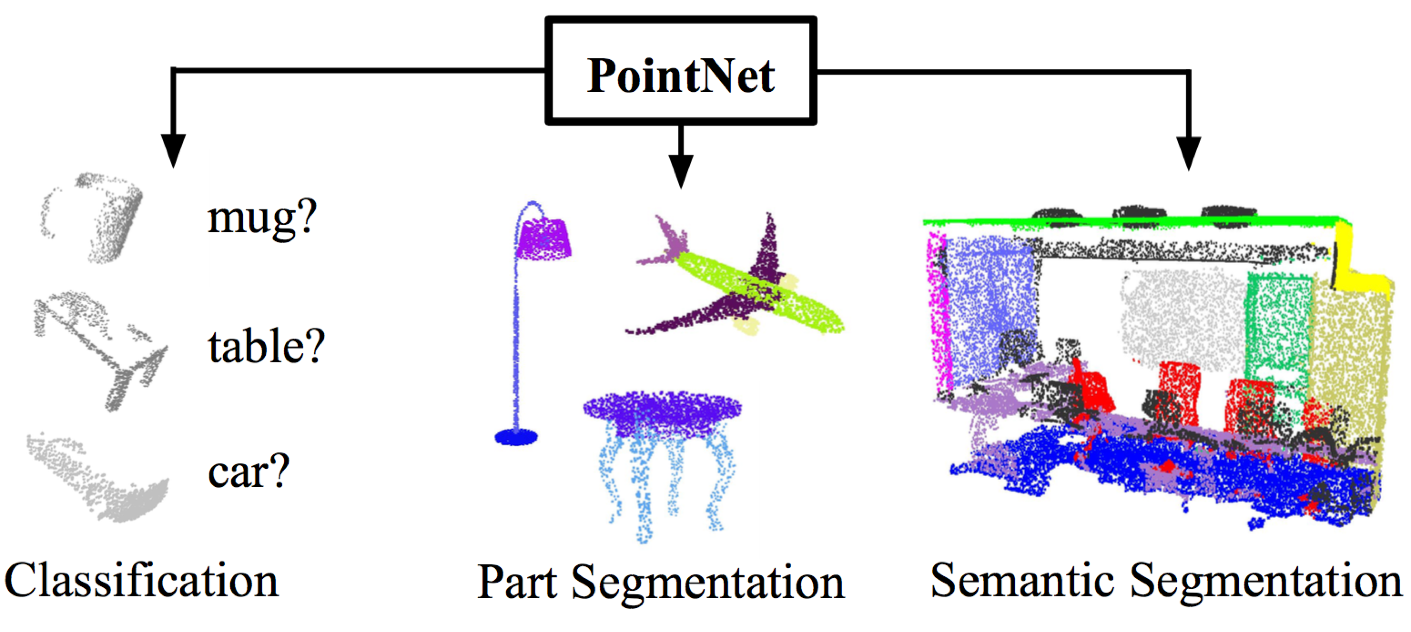
\includegraphics[width=0.5\textwidth]{p12_29}
    \end{multicols}
    \blfootnote{Figure from \cite{qi2017pointnet}.}
\end{frame}


\begin{frame}[c]
    \Huge
    \begin{columns}
        \column{0.65\textwidth}
        \begin{centering}
            What are your Questions?
        \end{centering}
        \column{0.35\textwidth}
        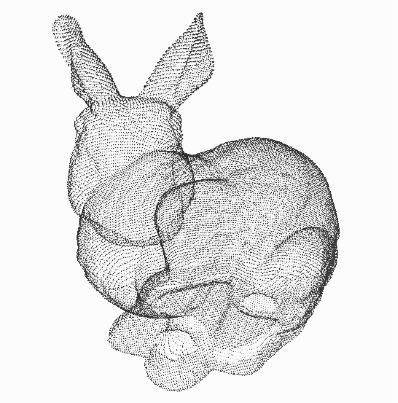
\includegraphics[width=\textwidth]{p04_12}
    \end{columns}
\end{frame}
